\documentclass[conference,compsoc]{IEEEtran}
\usepackage{graphicx}
\usepackage{cite}
%\usepackage[latin1]{inputenc}
\usepackage[english]{babel}
\usepackage{booktabs} % For improved table formatting
\usepackage{array} % For improved column formatting
\usepackage{multicol} % For multi-column formatting
\usepackage{url}
\usepackage{lipsum}



\begin{document}

\title{LIGHTWEIGHT APPROACHES IN BLOCK CRYPTOGRAPHY: A SURVEY}

\author{\IEEEauthorblockN{Fernando Ramirez Arredondo}
\IEEEauthorblockA{School of Computer Science\\
Universidad Católica San Pablo\\
Email: fernando.ramirez@ucsp.edu.pe}
}

\maketitle
\begin{abstract}
Lightweight Cryptography (LWC) is an expanding field of research as a result of its importance in providing security, via encrypting sensitive information, for IoT devices and other systems where traditional cryptography would be impractical due to resource demands. It is for this reason that several LWC primitives have been proposed. Among these, lightweight block ciphers are the most popular in terms of methods proposed and usage. These symmetric cryptographic algorithms operate on fixed-size blocks of data and transform each block independently into an output block of the same size. This work surveys 16 lightweight block ciphers' algorithms for resource-constrained devices, which have become increasingly important in today's world for their wide range of useful applications, from convenience and efficiency in our daily routines to far-reaching applications in healthcare, industry, and urban planning. The goal of this work is to provide a comprehensible classification of these methods in terms of their underlying structure,half of the selected LWC algorithms make use of some variation of a Feistel structure while the other half apply Substitution-Permutation networks,  followed by an accurate explanation of the tradeoff between these two when working with limited resources.
\end{abstract}

\begin{IEEEkeywords} Lightweight cryptography (LWC), Lightweight block ciphers, Resource-constrained devices, IoT, Feistel, Substitution-permutation network (SPN)\end{IEEEkeywords}

\section{Introduction}
Back in 2016, World Economic Forum founder and executive chairman Klaus Schwab wrote a book titled The Fourth Industrial Revolution, in which he explained that the way we live, work and relate to one another was about to be fundamentally altered by a digital revolution unlike the ones humanity had experienced before. Back to today, this so-called fourth industrial revolution has been characterized by a fusion of technologies that is blurring the lines between the physical, digital, and biological spheres\cite{WorldEconomicForum}.
The Internet of Things (IoT) paradigm corresponds to the inter-device domain created by devices embedded with electronics, software, sensors, and connectivity, enabling the transmission, receiving, and processing of data through various communication infrastructures. IoT generates more opportunities for direct integration between the physical world and computer-based systems.
As of 2019, IoT, which used to operate in smaller network spaces, has expanded to wide area networks, thereby increasing associated risks due to the expected surge in IoT devices in diverse environments. With the rapid growth of IoT applications, a substantial amount of sensitive data is generated and exchanged, leading to the observation of several security and privacy issues. As devices become more interconnected, security and privacy concerns will become more pronounced, continuously exposing additional security flaws and weaknesses. In statistical terms, all exposed errors and weaknesses may be exploited in an environment with billions of devices.

Thakor et al. categorized IoT devices into two groups based on their resources\cite{IoT_1}. The first group includes devices abundant in resources like servers, personal computers, tablets, smartphones, etc. The second group comprises devices limited in resources, such as industrial sensors or sensor nodes, RFID tags, actuators, etc.
This last group of devices face multiple constraints, including limitations in resources, memory, power/energy consumption, and speed. The challenge in terms of performance arises when attempting to implement traditional cryptography in devices with limited resources. This difficulty is attributed to the intricate and resource-intensive mathematical operations involved in traditional cryptographic techniques. Such operations require substantial memory space and demand high processing power. Moreover, the implementation cost of traditional cryptography in low-resource devices is notably high. Consequently, lightweight cryptography was introduced to address these issues. Lightweight cryptography, born out of the remarkable expansion in emerging ubiquitous technologies, represents a modern cryptographic technique.

Ciphers are categorized as either asymmetric or symmetric. While asymmetric ciphers provide enhanced security features, they require more computational power and tend to be relatively more costly. It is for this reason that asymmetric ciphers are not popular in the context of resource-constrained devices. Block ciphers and stream ciphers are the two main classifications of symmetric ciphers. This study specifically centers on block ciphers and endeavors to categorize them based on their inherent structural characteristics. 

\begin{table}[ht]
    \centering
    \caption{Table of Abbreviations}
    \begin{tabular}{ll}
        \toprule
        \textbf{Abbreviation} & \textbf{Definition} \\
        \midrule
        IoT & Internet of Things \\
        RFID & Radio Frequency IDentification \\
        WSN & Wireless Sensor Network \\
        LWC & LightWeight Cryptography \\
        LWHF & LightWeight Hash Function \\
        LWMAC & LightWeight Message Authentication Code \\
        LWSC & LightWeight Stream Cipher \\
        LWBC & LightWeight Block Cipher \\
        SPN & Substitution-Permutation Network \\
        FN & Feistel Network \\
        FPGA & Field-Programmable Gate Array \\
        GE & Gate Equivalents \\
        S-box & Substitution box \\
        P-box & Permutation box \\
        $f$ & Function \\
        AES & Advanced Encryption Standard \\
        LED & Light Encryption Device \\
        DULBC & Dynamic Ultra-Lightweight Block Cipher \\
        HIGHT & High security and lightweight \\
        DESL & Data Encryption Standard Lightweight \\
        NIST & National Institute of Standards and Technology (USA) \\
        RAM & Random-Access Memory \\
        ROM & Read-Only Memory \\
        XOR & eXclusive OR \\
        LFSR & Linear Feedback Shift Register \\
        \bottomrule
    \end{tabular}
    \label{table:abbreviations}
\end{table}
\section{Lightweight Cryptography (Theorical foundations)}
In Fan et al.'s study\cite{fan2013wg}, a lightweight cipher was defined as a cryptographic algorithm designed specifically for devices with limited resources. The algorithm needed to tackle three key challenges: minimizing overhead (in terms of silicon area or memory footprint), ensuring low-power consumption, and maintaining a sufficient level of security.

Other researchers have adopted a quantitative approach to the definition of lightweight ciphers. For instance, in the study conducted by Cazorla et al.\cite{cazorla2013survey} specific criteria were proposed for categorizing a cipher as lightweight. These criteria encompass attributes such as block size, key size, operations, and key scheduling. In the context of lightweight block ciphers, the term "lightweight" denotes a reduced block size (32, 48, or 64 bits) in contrast to conventional ciphers, which typically feature larger block sizes (64 or 128 bits).

NIST IR 8114 report on Lightweight Cryptography\cite{NIST}, working towards the standardization of
these algorithms, defines LWC as a subfield of cryptography that aims to provide solutions tailored for resource-constrained devices. This survey will follow NISTs standardization of lightweight algorithms, replicating its lightweight cryptographic primitives anatomy. Refer to Fig.\ref{fig:taxonomy} for the classification. 

\begin{figure*}
    \centering
    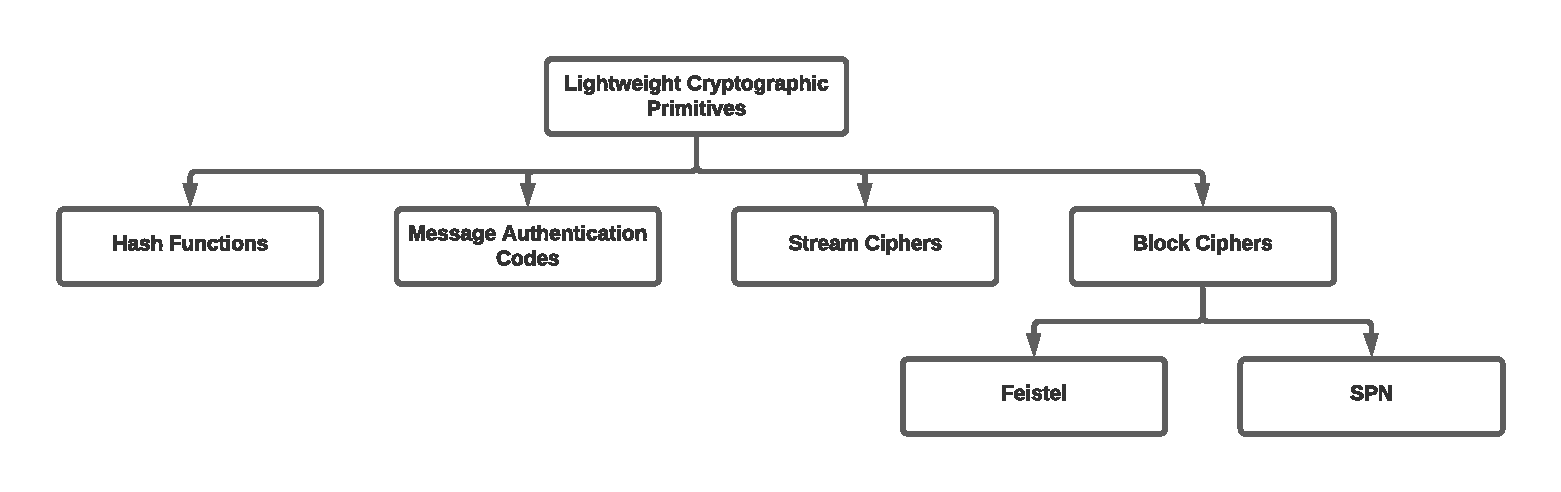
\includegraphics[width=\textwidth]{../figures/taxonomy.pdf}
    \caption{Structure-wise classification of LWC.}
    \label{fig:taxonomy}
\end{figure*}

\textbf{Lightweight hash functions} are defined as functions that take an arbitraty lenght input and output a fixed-sized value. While not as well-researched as block ciphers, have received a lot atention in the last few years, mainly due to the need of new and better equiped primitives as attacks on standardized primitives are increasingly common. A detailed description of LWHFs problematics and proposed solutions is done by Guo et al. in their presentation of PHOTON, a lightweight hash-function family\cite{guo2011photon}.

\textbf{Lightweight message authentication codes} generate a tag from a message and a secret key, which is used to verify the authenticity and the integrity of the message, preventing unauthorized and corrupted messages from being forwarded in a network. Roy et al. describe the inherent energy limitations in WSNs that make traditional implementations unaffordable in their presentation of LMAC, a LWMAC aimed for resource-constrained devices\cite{chowdhury2015lmac}.

While, as discused previously, LWBC are the main focus when working with resource-constrained devices, \textbf{lightweight stream ciphers} are used to secure the communication in applications where the plaintext length is either unknown or continuous, like network streams. Manifavas et al.\cite{manifavas2016survey} explain the advantages of implementing LWSC in applications pertaining to resource-constrained, aswell as problematics presented when cryptanalysed.

Several \textbf{lightweight block ciphers} have been suggested to gain performance advantages compared to traditional cryptographic methods. Certain ciphers achieved this by simplifying well-established block ciphers, enhancing their efficiency. Notable examples include AES-128\cite{AES-128}, a variant of NIST's Advanced Encryption Standard (AES), and DESL\cite{DESL}, which is a modified version of DES. In DESL, the round function and permutations were reduced to enhance hardware implementation efficiency.
On the other hand, some algorithms are dedicated block ciphers crafted from the ground up. An early example is PRESENT\cite{PRESENT}, specifically designed for resource-constrained hardware environments. Additionally, there are families of lightweight block ciphers such as SIMON and SPECK\cite{SIMONSPECK}. These were created to be simple, adaptable, and to deliver optimal performance in both hardware and software implementations.
The advantages in performance seen in lightweight block ciphers compared to traditional block ciphers result from design decisions that prioritize smaller block sizes, reduced key sizes, simpler rounds, more straightforward key schedules, and minimal implementations. 

Smaller block sizes in lightweight block ciphers, such as 64 or 80 bits compared to AES's 128 bits, are employed to optimize memory. However, it's crucial to recognize that the use of smaller block sizes imposes restrictions on the maximum number of plaintext blocks that can be encrypted. 

Smaller key sizes, less than 96 bits, are implemented in lightweight block ciphers for efficiency (e.g., 80-bit PRESENT), measured in terms of power consumption.

Simpler key schedules are a priority in lightweight block ciphers to mitigate the increased memory, latency, and power consumption associated with complex implementations. However, the choice for simplicity introduces potential vulnerabilities to attacks involving related keys, weak keys, known keys, or chosen keys.

Simpler rounds are featured in lightweight block ciphers with less complex components and operations compared to traditional block ciphers. In designs utilizing S-boxes, a preference for 4-bit S-boxes over 8-bit ones is observed, resulting in significant area savings. For example, the 4-bit S-box in PRESENT required 28 GEs, whereas the AES S-box needed 395 GEs. Hardware-oriented designs may opt for bit permutations (as in PRESENT) or recursive MDS matrices (as in LED\cite{LED}) instead of intricate linear layers. It's noteworthy that simpler rounds may necessitate more iterations to achieve the desired level of security.

Two lines of action have been employed to offer lightweight cryptographic primitives. The first involves creating efficient, cost-effective implementations for established and trusted algorithms, primarily focusing on block ciphers like AES. The second approach entails developing novel ciphers with the aim of minimizing hardware implementation costs, exemplified by the Simon and Speck families\cite{SIMONSPECK}.
\subsection{Target Devices}
Lightweight cryptography is designed to cater to a diverse range of devices and can be applied across a wide array of hardware and software configurations (See Table \ref{table:crypto_devices}). At the upper echelon of this device spectrum are servers and desktop computers, succeeded by tablets and smartphones. Traditional cryptographic algorithms typically exhibit satisfactory performance on these higher-end devices, making lightweight algorithms unnecessary for these platforms. However, at the lower end of the spectrum, we encounter devices like embedded systems, RFID devices, and sensor networks. It is in these highly constrained environments that lightweight cryptography takes center stage, addressing the specific needs of devices in this category\cite{NIST}.

\begin{table}[ht]
    \centering
    \caption{Cryptographic Approaches on Different Devices}
    \begin{tabular}{ll}
        \toprule
        \textbf{Device} & \textbf{Cryptography} \\
        \midrule
        Servers, Desktops and Smartphones & Conventional Cryptography \\
        Embedded Systems and RFID & Lightweight Cryptography \\
        \bottomrule
    \end{tabular}
    \label{table:crypto_devices}
\end{table}

While lightweight cryptography is primarily designed for devices at the lower end of the device spectrum, it's crucial to acknowledge the potential necessity of implementing lightweight algorithms at the higher end of the spectrum as well. For instance, even though many resource-constrained sensors may transmit data to an aggregator that, by most standards, is not constrained, the aggregator must still accommodate lightweight algorithms to interact effectively with the constrained sensors utilizing lightweight cryptographic methods. In essence, the decision on whether conventional standards are acceptable should consider the specific environment and application. The demand for lightweight cryptography arises not only from the limitations of a particular device but also from the need to ensure compatibility with other devices directly interacting within the application.
\subsection{Applications and Architectures}
IoT systems offer a wide range of services, including Intelligent Transportation Systems (ITS), smart grids, smart buildings, smart cities, e-Health, intelligent drug delivery systems, and more. Even Cyber-Physical Systems (CPS), such as Nuclear Power Plants (NPP), are encompassed within the IoT framework. The majority of these services are of a critical nature. Each IoT system is tailored to deliver a specific service, and for each application, diverse architectures are in development. 
Nevertheless, the shared drawbacks among many proposed architectures prevent them from fully meeting all IoT requirements. The applications can be classified into various domains, including Medical, Military, Industrial, Automobile, Environmental, Agriculture, Retail, and Consumer. Each domain offers its unique advantages while simultaneously tackling the IoT-related challenges discussed earlier.
\subsection{Performance Metrics} 
In the domain of designing cryptographic algorithms, there is a delicate equilibrium between the attained performance and the resources necessary to uphold a particular security level. Factors influencing performance include power and energy consumption, latency, and throughput.
Power and energy consumption are crucial metrics for constrained devices. Devices relying on harvested power, such as RFID chips utilizing electromagnetic fields, emphasize the significance of power considerations. In battery-operated devices with fixed energy stores, the concept of energy consumption gains prominence, especially when batteries are challenging or impossible to recharge or replace post-deployment.
Latency assumes special significance in specific real-time applications, being defined as the time gap between initiating an operation and generating its output. For example, in the realm of encryption, latency represents the interval from the initial request to encrypt plaintext to the reception of the corresponding ciphertext in the response.
Throughput pertains to the pace at which new outputs, such as authentication tags or ciphertext, are created. Unlike conventional algorithms, prioritizing high throughput may not be the main focus in lightweight designs. Nevertheless, a moderate level of throughput remains essential for most applications.

In hardware implementations, resource needs are commonly measured in terms of gate area, gate equivalents, or logic blocks. In software environments, these considerations are reflected in the utilization of registers, RAM, and ROM. These resource requirements are frequently labeled as costs, as increasing the number of gates or memory tends to raise the overall production cost of a device\cite{NIST}\cite{IoT_1}.
\subsubsection{Hardware-Specific Metrics} 
Resource needs for hardware platforms are commonly expressed in terms of gate area, measured in \(\mu \text{m}^2\). This area can be specified in logic blocks for field-programmable gate arrays (FPGAs) or in gate equivalents (GEs) for application-specific integrated circuit (ASIC) implementations.
In the realm of FPGAs, a logic block serves as the fundamental reconfigurable unit, housing various components like look-up tables (LUTs), flip-flops, and multiplexers.
For ASICs, one GE corresponds to the area required by a two-input NAND gate. The GE count is determined by dividing the area in \(\mu \text{m}^2\) by the area of the NAND gate.
\subsubsection{Software-Specific Metrics} 
In software applications, the assessment of resource needs involves considering the number of registers, RAM, and ROM bytes required. Functions with fewer registers experience lower calling overhead. ROM stores program code and fixed data, while RAM holds intermediate values for computations. This presents trade-offs between on-demand value calculation and referencing precomputed values.
\subsection{Security Analysis Techniques}
Cryptographic algorithms undergo diverse tests to confirm their efficiency. Within this study, we will provide a broad overview of the five most widely used cryptanalysis techniques.
\subsubsection{Linear Cryptanalysis} 
This attack is also referred to as a plaintext attack, and it is considered a basic attack. It relies on the occurrence of high probability linear expressions where plaintext bits, ciphertext bits, and subkeys are accountable\cite{matsui1993linear}.
\subsubsection{Differential Cryptanalysis} 
In this attack, the identification of trails is achieved through the utilization of a difference distribution table (DDT). The construction of the DDT is facilitated by high-probability input and output differences\cite{heys2002tutorial}.
\subsubsection{Zero Correlation Attack} 
In the zero correlation attack, we modify a single input bit and determine the corresponding ciphertext according to predefined rules.\cite{zero}
\subsubsection{Biclique Attack} 
This attack is a theoretical approach that determines the data complexity and computational complexity of the cipher. The Biclique attack is an extension of the meet-in-the-middle attack (MITM)\cite{jeong2012biclique}.
\subsubsection{Avalanche Effect Attack} 
The avalanche effect demonstrates the randomization nature of the cipher and its robust cryptanalytic properties, ensuring that under any circumstances, predicting the input plaintext is not feasible\cite{muthavhine2018analysis}.
\subsection{Classification of Attacks}
Attacks on IoT are divided into two modules\cite{NIST}.
\subsubsection{Protocol-Based Attacks} 
These types of attacks exploit the internal protocol-based structure of IoT components, impacting the communication medium and the forwarding channels of embedded systems.
\subsubsection{Data-Based Attacks} 
Data-based attacks encompass threats related to the original data packets and messages traversing through node sites. Security vulnerabilities such as hash collisions, denial-of-service (DoS) attacks, malicious node virtual machine creation, and data exposure are among the most impactful exploits in this category.

\section{Classification of Lightweight Block Ciphers}

\begin{table*}[ht]
    \label{table:ciphers}
    \centering
    \caption{Lightweight Block Ciphers}
    \begin{tabular}{lllll} 
     \toprule
     Algorithm & Key size & Block size & Structure & N. of rounds \\ 
     \midrule
     AES-128 (Daemen and Rijmen, 1999)\cite{AES-128}\cite{AES} & 128 & 128 & SPN & 10 \\ 
     mCrypton (Lim and Korkishko, 2005)\cite{MCRYPTON} & 64/96/128 & 64 & SPN & 12 \\
     PRESENT (Bogdanov et al., 2007)\cite{PRESENT} & 80/128 & 64 & SPN & 31 \\
     LED (Guo et al., 2011)\cite{LED} & 64/128 & 64 & SPN & 32/48 \\
     Hummingbird-2 (Engels et al., 2012)\cite{HUMMINGBIRD2} & 256 & 16 & SPN & 4 \\
     PRINCE (Borghoff et al., 2012)\cite{PRINCE} & 128 & 64 & SPN & 12 \\
     GIFT (Banik et al., 2017)\cite{GIFT} & 128 & 64/128 & SPN & 28/40 \\
     DULBC (Yang et al., 2022) \cite{DULBC} & 64/128 & 64 & SPN & 25/30 \\
     HIGHT (Hong et al., 2006)\cite{HIGHT} & 128 & 64 & Feistel & 32 \\
     DESL (Leander et al., 2007)\cite{DESL} & 54 & 64 & Feistel & 16 \\
     LBlock (Wu and Zhang, 2011)\cite{LBLOCK} & 80 & 64 & Feistel & 32 \\
     TWINE (Suzaki et al., 2012)\cite{TWINE} & 80-128 & 64 & Feistel & 36 \\
     GOST 28147-89 (Courtois, 2012)\cite{GOST} & 256 & 64 & Feistel & 32 \\
     QTL (Li et al., 2016)\cite{QTL} & 64/128 & 64 & Feistel & 16/20 \\
     SLIM (Aboushosha et al., 2020)\cite{SLIM} & 80 & 32 & Feistel & 32 \\
     SHADOW (Guo et al., 2021)\cite{SHADOW} & 64/128 & 32/64 & Feistel & 16/32 \\
     \bottomrule
    \end{tabular}
\end{table*}

This study surveys 16 LWBCs and categorizes them based on their underlying structures. Refer to Table (\ref{table:ciphers}) for a comprehensive list of the examined primitives, detailing their key sizes, block sizes, and the number of rounds. The majority of these ciphers operate with 64-bit plaintext blocks, as the encryption of large volumes of data is often unnecessary or even unfeasible in the context of most compact computing devices. The number of rounds is often related to the key size and its capacity to provide subkeys. Increasing the number of rounds represents a tradeoff between security and performance, a decision often influenced by the complexity of the cipher and the requirement for sufficient security. All these lightweight characteristics make these ciphers optimal when implemented in resource-constrained applications.

\begin{figure*}
    \centering
    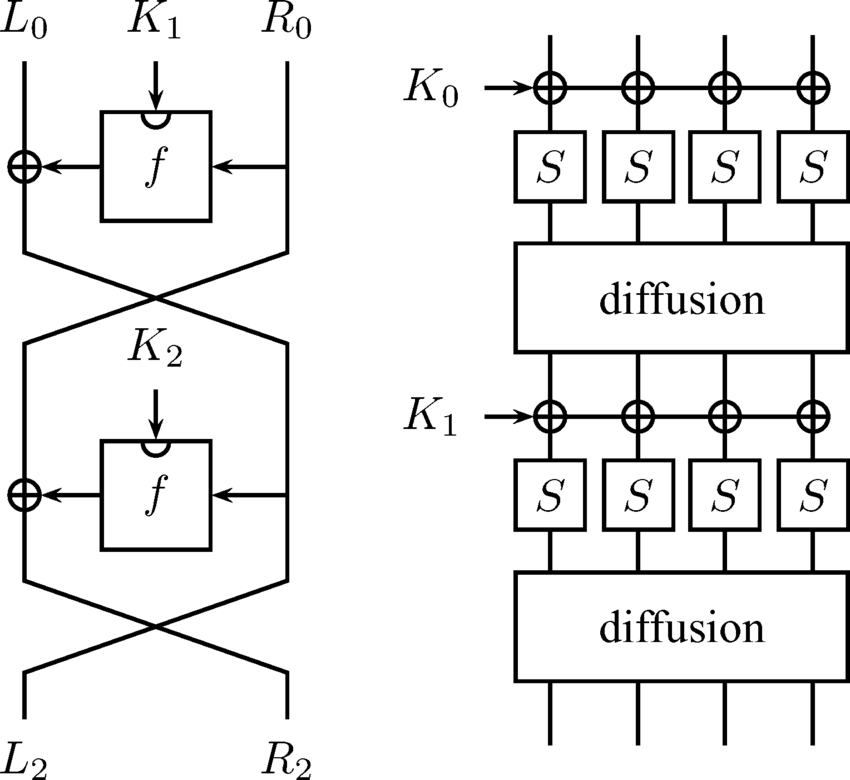
\includegraphics[width=\columnwidth]{../figures/FEISTEL-SPN.png}
    \caption{Representation of a Feistel Network (left) and a Substitution-Permutation Network (right).}
    \label{fig:FEISTEL-SPN}
\end{figure*}

\subsection{Substitution-Permutation Network }

A Substitution-Permutation Network operates by taking a block of plaintext and the key as inputs. It then undergoes multiple rounds or layers of alternating S-boxes and P-boxes to generate the corresponding ciphertext block. Typically, these transformations involve operations that are hardware-efficient, such as XOR and bitwise rotation. To decrypt, the process is reversed by employing the inverses of the S-boxes and P-boxes, and applying the round keys in reverse order\cite{heys1996substitution}. Refer to Fig. \ref{fig:FEISTEL-SPN} for a representation of a standard SPN and its components, including S (S-box), diffusion (P-box), and the corresponding subkey $K_n$ for 'n' representing each round. The rest of the section details the surveyed ciphers that share this structure.

\textbf{AES-128} is one of the three versions of the Rijmen and Daemen Advanced Encryption Standard (AES). This cipher is defined by a key size of 128 bits, a fixed block size of 128 bits, and 10 cycles of repetition. This last characteristic is particular to the key size. The encryption process involves applying subbyte, shift-rows, mixcolumn, and addroundkey operations within a 4x4 matrix of 128-bit blocks.

\textbf{mCrypton} is a variant of Crypton, characterized by its 64 bits block size and variable key size. This cipher operates on a 4x4 nibble array in which executes nibble-wise substitution, column-wise bit permutation, column-to-row transposition and key addition operations. The encryption process entails repeating this round transformation 12 times. The decryption process closely mirrors the encryption process but utilizes a distinct key schedule.

\textbf{PRESENT} has a block length of 64 bits and supports 80- and 128-bit keys. This cipher consists of 31 rounds involving addRoundKeys, sBoxLayer, and pLayer operations. The cipher employs a single 4-bit-to-4-bit S-box and a straightforward P-box designed for efficiency in implementation.

\textbf{LED} is a 64-bit block cipher with two primary instances using 64- and 128-bit keys. The cipher involves applying AddConstants, SubCells, ShiftRows, and MixColumnsSerial operations. Four rounds of operations are repeated either eight or twelve times, depending on the key size, with each set of round separated by an AddRoundKey operation.

\textbf{Hummingbird-2} succeeds Hummingbird and, unlike existing (ultra-)lightweight cryptographic primitives typically classified as either block ciphers or stream ciphers, represents a combination of both cipher structures. It has a 16-bit block size and a 128-bit key size. This encryption algorithm is structured with four 16-bit block ciphers and four 16-bit internal state registers. The encryption process begins by dividing the key into four 64-bit subkeys, which are then utilized in the block ciphers. It executes each set of operations, completing four rounds and generating the ciphertext.

\textbf{PRINCE} is a block cipher with a 64-bit block size and a 128-bit key that is divided into two 64-bit parts and extended to 192 bits. The cipher undergoes a total of 12 rounds. Each round includes key addition, an S-box layer, a linear layer, and the incorporation of a round constant. The cipher employs a 4-bit S-box, a 64x64 matrix, and a shift row operation reminiscent of AES.

\textbf{GIFT} is a 128-bit key cipher with block sizes of 64 and 128 bits, conducting 28 and 40 rounds, respectively. Each round of GIFT involves SubCells, PermBits, and AddRoundKey operations. Both versions of GIFT use the same invertible 4-bit Sbox, and the permutation is adjusted to accommodate twice as many state bits for the 128-bit block version.

\textbf{DULBC} has a plaintext block size of 64 bits, supporting both 80- and 128-bit keys. The number of rounds is 25 for the 80-bit key variant and 30 for the 128-bit key variant, which includes a round of 'whitening' operation with the round keys. Each round consists of S-box layer, MixColumns, AddConstants, and AddRoundKeys operations, followed by a bit permutation.


\subsection{Feistel Network} 

A Feistel Network employs a round function, a mechanism that takes two inputs, a data block and a subkey, and produces an output of identical size to the data block. During each round, the round function is applied to half of the data intended for encryption, and the resulting output is XORed with the other half of the data. This process is iterated a predetermined number of times, culminating in the encrypted data as the final output\cite{FEISTEL}. Refer to Fig \ref{fig:FEISTEL-SPN} for a representation of a standard Feistel Network (FN) and its round functions, denoted as $f$, receiving the data block $R_n$, representing the rightmost part of the full input, and the subkey $K_n$ for n representing each round. $L_n$ represents the left part of the input. The rest of the section details the surveyed ciphers that share this structure.

\textbf{HIGHT} features a 64-bit block length and a 128-bit key length. A characteristic of this cipher is its utilization of elementary operations like XOR, and left bitwise rotation. The encryption process starts with an initial transformation, proceeds through 32 rounds of operations, and concludes with a final transformation.

\textbf{DESL}, which is based on the classical DES design, encrypts one 64-bit block of plaintext using a 54-bit key but unlike DES it uses a single S-box for every one of its 16 rounds and ommitts the initial permutation and its inverse.

\textbf{LBlock} has a block length of 64 bits and a key length of 80 bits. The encryption algorithm of LBlock consists of a 32-round iterative structure, which is a variant of a FN. This structure is formed by a round function, confusion function, and diffusion function.

\textbf{TWINE} is a 64-bit block cipher characterized by the absence of a Galois-Field matrix, bit permutation, and the use of components such as a 4-bit S-box, XOR, and 4-bit-wise permutation (shuffle). Both 80- and 129-bit key implementations perform 36 rounds of a Type-2 FN with 16 nibble-blocks.

\textbf{GOST} is a cipher characterized by a straightforward FN, featuring a block size of 64 bits, 256-bit keys, and 32 rounds. Every iteration executes a key addition , a group of 8 bijective S-boxes operating on 4 bits, and a basic rotation of 11 positions. 

The \textbf{QTL} block cipher, with a block size of 64 bits, accommodates both 64- and 128-bit keys with 16 and 20 rounds, respectively. Its main strength is that it addresses the slow diffusion of traditional Feistel-type structures by employing a variant of a generalized FN.

In \textbf{SLIM}, the input undergoes division into right and left parts, traversing 32 rounds alongside the corresponding sub-keys. The block size is 32 bits, and the key size is 80 bits. Each round structure consists of XOR, S-box, and permutation.

\textbf{Shadow} employs a generalized FN with a 4-branch configuration, featuring a 32-bit block size with a 64-bit key and a 64-bit block size with a 128-bit key. It operates with 16 and 32 rounds for the respective version of the cipher. This cipher makes user of AND, Rotation, and XOR operators.

 
\section{Strengths and Weaknesses}
\textbf{Strengths.} Feistel Networks boast a robust theoretical basis, with extensively researched and established security properties. They are characterized by their simplicity in design, facilitating comprehension and analysis. Additionally, their structure allows for straightforward parallelization of encryption and decryption processes, resulting in accelerated implementations.
On the other hand, Substitution-Permutation Networks have demonstrated notable resilience against differential cryptanalysis, a prevalent attack method. Efficiency extends to both hardware and software implementations, thanks to their structure that supports parallelization.

\textbf{Weaknesses.} Both these architectures often involve intricate key schedules, particularly in designs such as AES-128. Feistel Networks demonstrate proficiency with specific block sizes, necessitating potential adjustments in design for different sizes. Certain Substitution-Permutation Network designs may display susceptibility to linear cryptanalysis, representing a possible vulnerability. Although efficient, these networks may demand increased resources in specific implementations\cite{FEISTEL}\cite{heys1996substitution}.


\section{Conclusions}
The Internet of Things (IoT) plays a crucial role in facilitating direct integration between the physical and digital realms. However, the rapid expansion of IoT, particularly in wide area networks, raises significant security and privacy concerns. Resource-constrained IoT devices, facing limitations in memory, power, and speed, pose a challenge for traditional cryptography due to its complexity and high implementation costs. To address this, lightweight cryptography has emerged as a modern solution tailored to the constraints of low-resource devices. This study focuses on categorizing block ciphers based on their structural characteristics. The studied ciphers share characteristics that make them optimal when implemented in resource-constrained applications. While some are scaled-down versions of other, more complex ciphers, others were designed from scratch to accommodate this lightweight paradigm. This scaling-down is defined as reducing block sizes, key sizes, the number of rounds, and even reducing the complexity of their functions.

Finally, the utilization of FNs and SPNs contributes significantly to the field of cryptography, addressing the challenges posed by resource-constrained environments. These cryptographic paradigms play a vital role in securing the ever-expanding landscape of interconnected devices and systems, ensuring a balance between security and efficiency in diverse computing scenarios.

\bibliographystyle{IEEEtran}
\bibliography{../bibliography/references}
\end{document}

